\section{配对随机实验与证据边界}
\label{sec:experiment}

\subsection{方法协议与可复现设置}

实验在 Apollo 路径--速度解耦规划环境中运行四种方法。B0-TimeBlind 在路径阶段只处理静态障碍物，使用固定裕度与逐障碍物贪心选向；B1-TimeAwareGreedy 加入到达时间查询，但仍使用固定裕度与逐障碍物选向；B2-IterativePVD 在 B1 上用上一轮速度曲线反推首次到达时刻，最多交替三轮；MIKU 使用时间查询、纵向分组、前缀最大间隙与差异化裕度。四者共享场景、障碍物预测、车辆尺寸、路径 QP、速度 QP、动力学上下界与规划时域。

运行环境为 Intel Core i9-14900HX（32 逻辑处理器）与 Linux 7.2.2，二次规划求解器为 OSQP 1.1.1\citep{stellato2020osqp}。全周期耗时从方法入口至返回计时，包含边界构造、DP、路径/速度 QP 及 B2 全部迭代，而非只计最后一次 QP。原始 CSV、参数开关、随机种子、失败清单与派生宏由同一入口生成，表格数值不手工转录。

\subsection{随机场景与指标}

实验包含行人横穿、车辆切入、停车车辆与对向动态障碍物、窄路多障碍物、多动态障碍物交织和预测含噪六类。每类使用从 0 开始的 \RandSeedCount 个固定种子，共 \RandCaseCount 个配对实例。含噪类对自车定位/速度以及障碍物位置/速度的规划输入施加扰动，安全评估始终使用未扰动真值。

安全性以直道 SL 坐标中自车与障碍物实体矩形的最小有符号边界距离、碰撞与最小 TTC 衡量。为区分 QP 边界接触与实体侵入，穿透深度超过 1\,mm 才计为碰撞，但有符号间距保留原值。无碰撞到达率要求轨迹到达 $s_{max}-1$\,m 且未碰撞。效率指标包含通行时间、平均速度、路径长度与进度比；舒适性包含纵/横向加速度和 jerk RMS。未无碰撞到达的样本在配对通行时间中记为场景时域加 5\,s，同时单独报告降级停车率，避免只在成功子集上产生生存者偏差。配对差值统一定义为 MIKU 减基线，95\% 置信区间由 5,000 次配对 bootstrap 得到，效应量为配对 Cohen $d_z$。

\subsection{主结果}

\begin{table}[htbp]
\centering
\caption{六类随机场景的全量汇总（每种方法 $n=\RandCaseCount$）}
\label{tab:random_overall}
\small
\begin{adjustbox}{max width=\textwidth}
\begin{tabular}{lrrrrrrrr}
\toprule
方法 & 无碰撞到达(\%) & 碰撞(\%) & 降级停车(\%) & 间距(m) & jerk RMS & P50(ms) & P95(ms) & P99(ms) \\
\midrule
B0 & \RandAllBZeroSuccessPct & \RandAllBZeroCollisionPct & \RandAllBZeroStopPct & \RandAllBZeroClearance & \RandAllBZeroJerkRms & \RandAllBZeroRuntimePfifty & \RandAllBZeroRuntimePninetyfive & \RandAllBZeroRuntimePninetynine \\
B1 & \RandAllBOneSuccessPct & \RandAllBOneCollisionPct & \RandAllBOneStopPct & \RandAllBOneClearance & \RandAllBOneJerkRms & \RandAllBOneRuntimePfifty & \RandAllBOneRuntimePninetyfive & \RandAllBOneRuntimePninetynine \\
B2 & \RandAllBTwoSuccessPct & \RandAllBTwoCollisionPct & \RandAllBTwoStopPct & \RandAllBTwoClearance & \RandAllBTwoJerkRms & \RandAllBTwoRuntimePfifty & \RandAllBTwoRuntimePninetyfive & \RandAllBTwoRuntimePninetynine \\
MIKU & \RandAllMikuSuccessPct & \RandAllMikuCollisionPct & \RandAllMikuStopPct & \RandAllMikuClearance & \RandAllMikuJerkRms & \RandAllMikuRuntimePfifty & \RandAllMikuRuntimePninetyfive & \RandAllMikuRuntimePninetynine \\
\bottomrule
\end{tabular}
\end{adjustbox}
\end{table}

MIKU 的无碰撞到达率为 \RandAllMikuSuccessPct\%，B0、B1 和 B2 分别为 \RandAllBZeroSuccessPct\%、\RandAllBOneSuccessPct\% 和 \RandAllBTwoSuccessPct\%。与 B0 的配对差值为 \RandAllMikuVsBZeroSuccessDiff 个百分点，95\% CI [\RandAllMikuVsBZeroSuccessCiLow,\RandAllMikuVsBZeroSuccessCiHigh]，$d_z=\RandAllMikuVsBZeroSuccessEffect$。但 MIKU 与 B0 的碰撞率都是 \RandAllMikuCollisionPct\%，碰撞率配对差值为 \RandAllMikuVsBZeroCollisionDiff 个百分点，95\% CI [\RandAllMikuVsBZeroCollisionCiLow,\RandAllMikuVsBZeroCollisionCiHigh]。因此数据支持的是汇总可达性差值，不是碰撞风险降低。

B2 包含多轮协调，其 P95 全周期耗时为 \RandAllBTwoRuntimePninetyfive\,ms；MIKU 为 \RandAllMikuRuntimePninetyfive\,ms。由于四种方法在同一进程中固定顺序运行，该墙钟结果用于描述当前硬件上的成本，不把 MIKU 与 B0 的小幅耗时差异解读为可迁移的速度优势。

\begin{figure}[htbp]
\centering
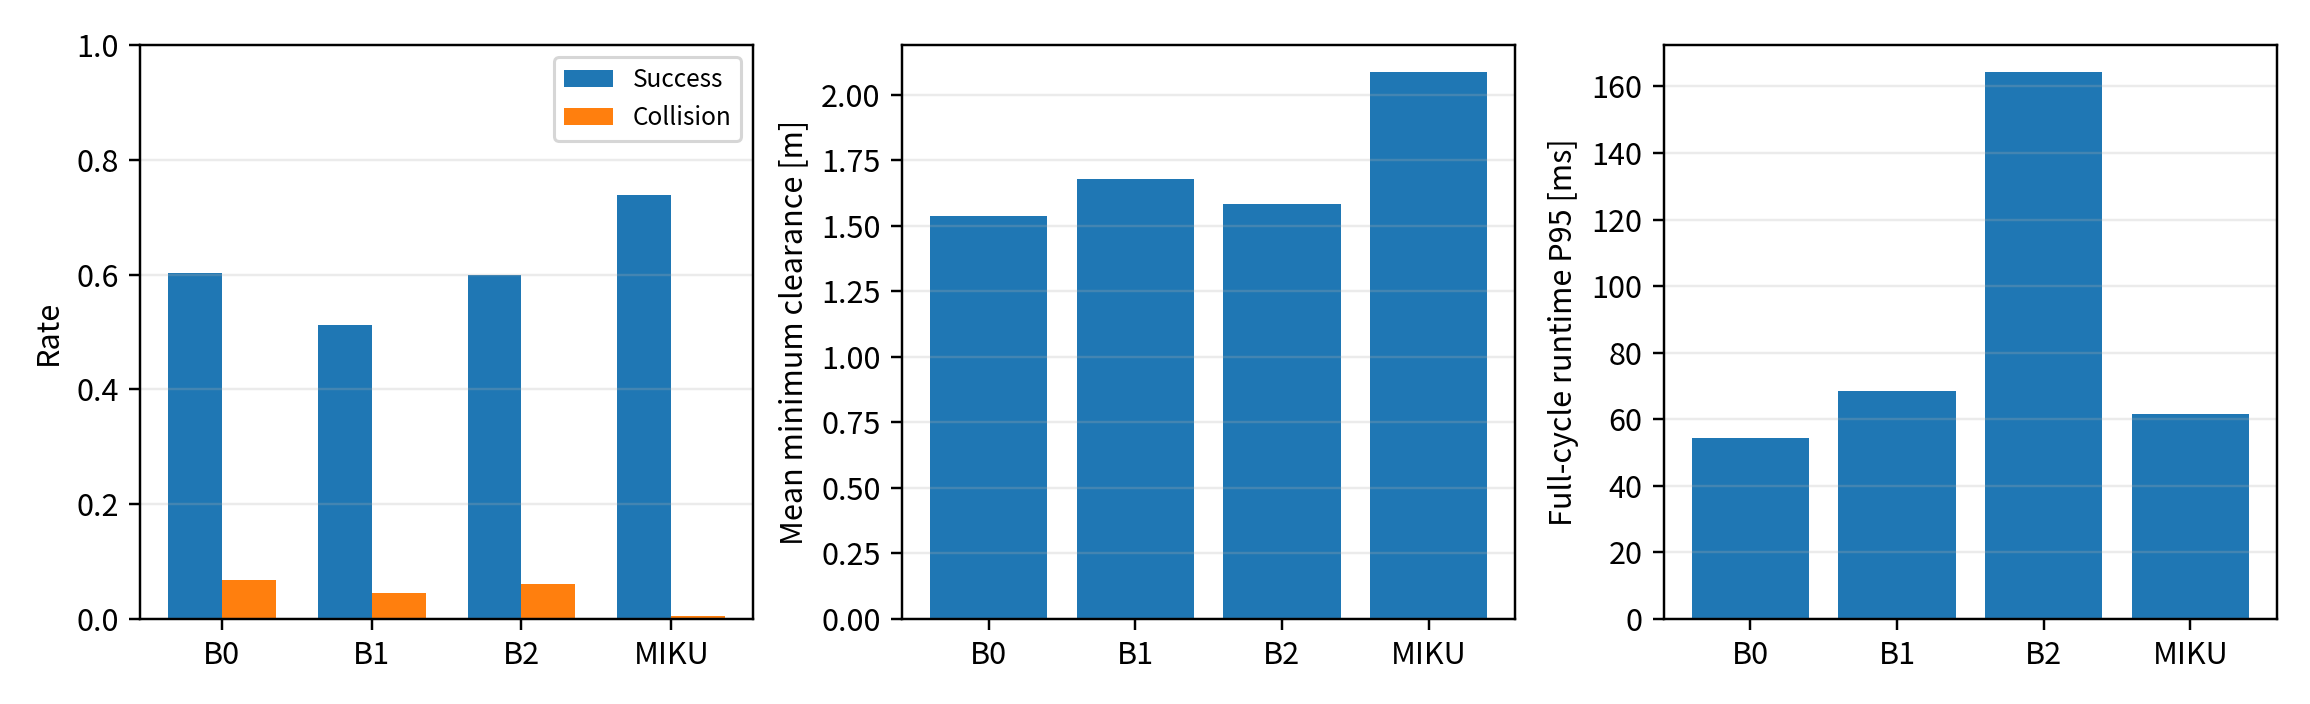
\includegraphics[width=0.96\textwidth]{generated/randomized_summary.png}
\caption{六类配对随机实验的汇总指标}
\label{fig:random_summary}
\end{figure}

\subsection{分场景差异与失效分析}

\begin{table}[htbp]
\centering
\caption{MIKU 与 B0 的分场景无碰撞到达率}
\label{tab:random_by_case}
\small
\begin{tabular}{lrrrr}
\toprule
场景 & B0(\%) & MIKU(\%) & 配对差(百分点) & 95\% CI \\
\midrule
行人横穿 & \RandCrossingBZeroSuccessPct & \RandCrossingMikuSuccessPct & \RandCrossingMikuVsBZeroSuccessDiff & [\RandCrossingMikuVsBZeroSuccessCiLow,\RandCrossingMikuVsBZeroSuccessCiHigh] \\
车辆切入 & \RandCutInBZeroSuccessPct & \RandCutInMikuSuccessPct & \RandCutInMikuVsBZeroSuccessDiff & [\RandCutInMikuVsBZeroSuccessCiLow,\RandCutInMikuVsBZeroSuccessCiHigh] \\
停车+对向车 & \RandParkedBZeroSuccessPct & \RandParkedMikuSuccessPct & \RandParkedMikuVsBZeroSuccessDiff & [\RandParkedMikuVsBZeroSuccessCiLow,\RandParkedMikuVsBZeroSuccessCiHigh] \\
窄路多障碍 & \RandNarrowBZeroSuccessPct & \RandNarrowMikuSuccessPct & \RandNarrowMikuVsBZeroSuccessDiff & [\RandNarrowMikuVsBZeroSuccessCiLow,\RandNarrowMikuVsBZeroSuccessCiHigh] \\
多动态交织 & \RandInterleavedBZeroSuccessPct & \RandInterleavedMikuSuccessPct & \RandInterleavedMikuVsBZeroSuccessDiff & [\RandInterleavedMikuVsBZeroSuccessCiLow,\RandInterleavedMikuVsBZeroSuccessCiHigh] \\
预测含噪 & \RandNoiseBZeroSuccessPct & \RandNoiseMikuSuccessPct & \RandNoiseMikuVsBZeroSuccessDiff & [\RandNoiseMikuVsBZeroSuccessCiLow,\RandNoiseMikuVsBZeroSuccessCiHigh] \\
\bottomrule
\end{tabular}
\end{table}

表~\ref{tab:random_by_case}显示汇总差异由窄路多障碍类驱动：该类中 MIKU 比 B0 高 \RandNarrowMikuVsBZeroSuccessDiff 个百分点，95\% CI [\RandNarrowMikuVsBZeroSuccessCiLow,\RandNarrowMikuVsBZeroSuccessCiHigh]。这与差异化裕度避免小尺寸锥桶与边界重复挤占通道的机制一致。相反，行人横穿与多动态交织类的配对差分别为 \RandCrossingMikuVsBZeroSuccessDiff 和 \RandInterleavedMikuVsBZeroSuccessDiff 个百分点，说明单次到达时间查询可在动态交织中选到不利的横向同伦类。这是方法的适用边界，而不是可通过汇总平均隐去的离群值。

含噪类中 MIKU 的无碰撞到达率为 \RandNoiseMikuSuccessPct\%，碰撞率为 \RandNoiseMikuCollisionPct\%，均明显差于无噪的车辆切入类。失败清单逐例保留种子、方法、进度比与最小间距；主要失效是时域内未到达/降级停车，而含噪类还暴露出预测偏差下安全裕度不足。

\subsection{联合参照与滚动重规划补充实验}

B3-JointReference 在 $(t,s,l,v,\dot l)$ 上同步搜索，公开网格分辨率依次为 0.5\,s、0.5\,m、0.25\,m、1.0\,m/s 与 0.5\,m/s，每层确定性保留至多 20,000 个状态。该方法与 MIKU 共享车辆实体尺寸、道路边界、纵向加减速和横向运动上限，但不使用顺序路径/速度 QP。由于它含 beam 截断且网格离散，只作为质量--开销参照，不称为连续全局最优。

\begin{table}[htbp]
\centering
\caption{小规模联合参照与滚动重规划补充结果}
\label{tab:supplementary_protocols}
\small
\begin{tabular}{llrrrr}
\toprule
协议 & 方法 & $n$ & 到达率(\%) & 碰撞率(\%) & P95耗时(ms) \\
\midrule
联合网格子集 & B3 & \JointCaseCount & \JointBThreeSuccessPct & \JointBThreeCollisionPct & \JointBThreeRuntimePninetyfive \\
联合网格子集 & MIKU & \JointCaseCount & \JointMikuSuccessPct & \JointMikuCollisionPct & \JointMikuRuntimePninetyfive \\
滚动重规划子集 & B0 & \ClosedCaseCount & \ClosedBZeroSuccessPct & \ClosedBZeroCollisionPct & \ClosedBZeroRuntimePninetyfive \\
滚动重规划子集 & MIKU & \ClosedCaseCount & \ClosedMikuSuccessPct & \ClosedMikuCollisionPct & \ClosedMikuRuntimePninetyfive \\
\bottomrule
\end{tabular}
\end{table}

在每类 5 个种子的 \JointCaseCount 个配对子集中，B3 与 MIKU 的无碰撞到达率分别为 \JointBThreeSuccessPct\% 和 \JointMikuSuccessPct\%，配对差为 \JointMikuVsBThreeSuccessDiff 个百分点（95\% CI [\JointMikuVsBThreeSuccessCiLow,\JointMikuVsBThreeSuccessCiHigh]）。B3 单独成功的配对有 \JointBThreeOnlySuccessCount 个，MIKU 单独成功的配对有 \JointMikuOnlySuccessCount 个；这些不一致个例提示顺序解耦可能遗漏联合搜索找到的轨迹，但由于两者保护带定义不同，不能把差异全部归因于解耦结构；跨零的置信区间也不支持总体差异声称。B3 的真值碰撞率为 \JointBThreeCollisionPct\%，MIKU 为 \JointMikuCollisionPct\%；B3 的 P95 完整搜索耗时为 \JointBThreeRuntimePninetyfive\,ms，MIKU 为 \JointMikuRuntimePninetyfive\,ms。粗网格和 0.10\,m 固定保护带不足以抵御含噪输入；B3 只是质量--开销参照，不是安全上界或连续全局最优解。

滚动实验对每类 10 个种子执行“规划 0.5\,s、更新自车与障碍物、再规划”，共 \ClosedCaseCount 个配对场景。MIKU 与 B0 的到达率分别为 \ClosedMikuSuccessPct\% 和 \ClosedBZeroSuccessPct\%，配对差为 \ClosedMikuVsBZeroSuccessDiff 个百分点（95\% CI [\ClosedMikuVsBZeroSuccessCiLow,\ClosedMikuVsBZeroSuccessCiHigh]）。两者碰撞率分别为 \ClosedMikuCollisionPct\% 和 \ClosedBZeroCollisionPct\%，差值为 \ClosedMikuVsBZeroCollisionDiff 个百分点（95\% CI [\ClosedMikuVsBZeroCollisionCiLow,\ClosedMikuVsBZeroCollisionCiHigh]），因而小样本到达率改善不能被解读为安全性改善。这里的耗时是单场景全部规划周期的累计墙钟时间；固定运行顺序和小样本使其只用于规模描述。总体到达率偏低，表明 0.5\,s 执行步长与有限场景时域下仍有大量停车/未到达，不能据此声称完整闭环性能成熟。

\subsection{消融决策与限制}

确定性机理消融显示，差异化裕度是窄路压力构型的活跃组件；关闭分组与最大间隙使密集施工的手工临界构型失败。但对该构型施加很小的几何扰动后，组级改善未保持，因而本文只把它作为机理证据。前缀最大间隙的精确性与该性能鲁棒性是两个不同命题：前者已由定理和 4,000 例穷举 oracle 支持，后者仍受场景分布与上游边界误差影响。

经修正的占用补集安全时窗能表达先通过和后通过，也通过了随机点集 oracle；但开启它后没有在当前压力场景中形成独立正收益，并在动静混合场景出现可重复回归。按预先规定的决策门，它已从主方法关闭，不作为性能贡献。

\subsection{灵敏度分析}

在 P1--P4 中每个场景对 5 个威胁度权重同时施加 $\pm\SensPerturbPct\%$ 均匀扰动并重新归一，每场景 100 次的安全裕度最大相对变化为 \SensWorstRelDev\%。另对每场景 \SensTrajectoryTrialCount 组权重扰动重新运行完整规划，80 条轨迹均到达终点，相对基准的最大横向偏移变化为 \SensOneTrajectoryMaxLateralDev\,m，终点进度和 jerk RMS 在报告精度下未变。这只支持权重局部稳定性：对 $\tau(s)$ 施加 $\pm20\%$、动态障碍物纵向速度施加 $\pm0.5$\,m/s、横向位置施加 $\pm0.2$\,m 的 \SensSingleFactorCount 个对称端点中，到达率仅为 \SensSingleFactorSuccessPct\%；两个动态压力场景的 \SensDynamicSingleFactorCount 个端点中仅为 \SensDynamicSingleFactorSuccessPct\%。因此方法对权重的局部稳定不能外推为对时序与预测误差的鲁棒性。

主实验是有限时域规划轨迹对真值预测的配对回放；补充滚动实验闭合了规划器状态更新，但仍不是实车路测，也未覆盖感知器、控制器与车辆执行器构成的系统闭环。B3 仅有 30 例且采用粗网格与 beam 截断。因此，这些数据只支持本文明示的随机生成分布与 Apollo 规划器在环结论，不支持对自然交通分布或实车安全性的外推。
